\documentclass[twoside]{article}
\setlength{\oddsidemargin}{0 in}
\setlength{\evensidemargin}{0 in}
\setlength{\topmargin}{-0.6 in}
\setlength{\textwidth}{6.5 in}
\setlength{\textheight}{8.5 in}
\setlength{\headsep}{0.75 in}
\setlength{\parindent}{0 in}
\setlength{\parskip}{0.1 in}

\usepackage{url}
\usepackage{titlesec}
\setcounter{secnumdepth}{3}
\usepackage{palatino}
\usepackage{marginnote}
\usepackage{multirow}
\usepackage{easybmat,bigdelim,arydshln}
\usepackage[authoryear,round]{natbib}
\usepackage{amssymb,amsmath,amsthm,amsfonts}
\usepackage{mathtools}
%\usepackage{nicematrix}
\usepackage{arydshln}
\usepackage{caption}
\usepackage{hyperref}
\usepackage{tcolorbox}
\tcbuselibrary{skins, breakable, theorems}
\usepackage{newpxtext,newpxmath}
\usepackage{longtable}
\usepackage{enumitem}
\makeatletter

\let\bar\overline

\setlist[itemize]{topsep=0pt,leftmargin=10pt,itemsep=-0.2em}
\usepackage{xcolor}
\usepackage{tikz}
\usepackage{pgfplots}
\pgfplotsset{compat = newest}
\usetikzlibrary{patterns,decorations.pathreplacing,decorations.markings,fit,shapes.geometric,angles,quotes,arrows}
\usepgfplotslibrary{fillbetween}

\usepackage{ifthen}
\usepackage{tikz-3dplot}

\pgfdeclarelayer{ft}
\pgfdeclarelayer{bg}
\pgfsetlayers{bg,main,ft}

\hypersetup{
    colorlinks,
    citecolor=red,
    filecolor=black,
    linkcolor=violet,
    urlcolor=blue
}

\definecolor{myblue}{cmyk}{1,.72,0,.38}
\definecolor{mypurple}{cmyk}{.57,1,0,.58}
\definecolor{myred}{cmyk}{0,.88,.88,.58}
\definecolor{mygreen}{cmyk}{1,0,.69,.66}
\definecolor{myorange}{cmyk}{0,.58,100,.20}
\definecolor{glaucous}{rgb}{0.38, 0.51, 0.71}

\makeatletter
\renewcommand{\thefigure}{\thesection.\arabic{figure}}
\newtheoremstyle{indented}
  {3pt}% space before
  {3pt}% space after
  {\addtolength{\@totalleftmargin}{3.5em}
   \addtolength{\linewidth}{-3.5em}
   \parshape 1 3.5em \linewidth}% body font
  {}% indent
  {\bfseries}% header font
  {.}% punctuation
  {.5em}% after theorem header
  {}% header specification (empty for default)
\makeatother

\newcommand{\ind}{\perp\!\!\!\perp}

\theoremstyle{definition}
\newtheorem{defin}{Definition}[section] % Creates a new counter, number within section
\newtheorem{prt}[defin]{Remark} 
\newtheorem{prts}[defin]{Remarks} % Again share defin's counter
\newtheorem{exmp}[defin]{Example} % etc.
\newtheorem{exmps}[defin]{Examples}
\newtheorem*{note}{Note}
\tcbuselibrary{theorems}

% use counter*=defin to make each tcbtheorem share defin's counter

\newtcbtheorem[use counter*=defin, number within=section]{definition}{Definition}{enhanced, breakable,
    colback = white, colframe = red!55!black, colbacktitle = red!55!black, attach boxed title to top left = {yshift = -2.5mm, xshift = 3mm}, boxed title style = {sharp corners},fonttitle=\bfseries}{def}

\newtcbtheorem[use counter*=defin, number within=section]{theorem}{Theorem}{enhanced, breakable,
    colback = white, colframe = blue!45!black, colbacktitle = blue!45!black, attach boxed title to top left = {yshift = -2.5mm, xshift = 3mm}, boxed title style = {sharp corners},fonttitle=\bfseries}{thm}
    
\newtcbtheorem[use counter*=defin, number within=section]{proposition}{Proposition}{enhanced, breakable,
    colback = white, colframe = teal, colbacktitle = teal, attach boxed title to top left = {yshift = -2.5mm, xshift = 3mm}, boxed title style = {sharp corners},fonttitle=\bfseries}{prop}

\newtcbtheorem[use counter*=defin, number within=section]{lemma}{Lemma}{enhanced, breakable,
    colback = white, colframe = orange!80!black, colbacktitle = orange!80!black, attach boxed title to top left = {yshift = -2.5mm, xshift = 3mm}, boxed title style = {sharp corners},fonttitle=\bfseries}{lemma}

\newtcbtheorem[use counter*=defin, number within=section]{example}{Example}{enhanced, breakable,
    colback = white, colframe = yellow!60!black, colbacktitle = yellow!60!black, attach boxed title to top left = {yshift = -2.5mm, xshift = 3mm}, boxed title style = {sharp corners},fonttitle=\bfseries}{exmp}

\newtcbtheorem[use counter*=defin, number within=section]{assumption}{Assumption}{enhanced, breakable,
    colback = white, colframe = violet!60!white, colbacktitle = violet!60!white, attach boxed title to top left = {yshift = -2.5mm, xshift = 3mm}, boxed title style = {sharp corners},fonttitle=\bfseries}{assump}

\newtcbtheorem[use counter*=defin, number within=section]{algorithm}{Algorithm}{enhanced, breakable,
    colback = white, colframe = green!55!black, colbacktitle = green!55!black, attach boxed title to top left = {yshift = -2.5mm, xshift = 3mm}, boxed title style = {sharp corners},fonttitle=\bfseries}{algm}
%\newtcolorbox{example}[1]{enhanced, breakable, colback = white, colframe = orange!85!black, colbacktitle = orange!85!black, attach boxed title to top left = {yshift = -2.5mm, xshift = 3mm}, boxed title style = {sharp corners},fonttitle=\bfseries, title={Example: #1}}

\newtcbox{\myhl}[1][white]
  {on line, arc = 0pt, outer arc = 0pt,
    colback = #1!20!white, colframe = #1!50!black,
    boxsep = 0pt, left = 1pt, right = 1pt, top = 1pt, bottom = 1pt, boxrule = 0pt, bottomrule =0pt, toprule =0pt}
    
\newtcbox{\myhlrule}[1][white]
  {on line, arc = 0pt, outer arc = 0pt,
    colback = #1!20!white, colframe = #1!50!black,
    boxsep = 0pt, left = 1pt, right = 1pt, top = 1pt, bottom = 1pt, boxrule = 0pt, bottomrule =0.5pt, toprule =0.5pt}
%
% The following commands set up the lecnum (lecture number)
% counter and make various numbering schemes work relative
% to the lecture number.
%
\newcounter{lecnum}
\renewcommand{\thepage}{\thelecnum-\arabic{page}}
\renewcommand{\thesection}{\thelecnum.\arabic{section}}
\renewcommand{\theequation}{\thelecnum.\arabic{equation}}
\renewcommand{\thefigure}{\thelecnum.\arabic{figure}}
\renewcommand{\thetable}{\thelecnum.\arabic{table}}

\newcommand{\sidenotes}[1]{\marginnote{\raggedright\scriptsize#1}}
%
% The following macro is used to generate the header.
%
\newcommand{\lecture}[6]{
   \pagestyle{myheadings}
   \thispagestyle{plain}
   \newpage
   \setcounter{lecnum}{#1}
   \setcounter{page}{1}
   \noindent
   \begin{center}
   \framebox{
      \vbox{\vspace{2mm}
    \hbox to 6.28in { {\bf Econometrics
	\hfill \today} }
       \vspace{4mm}
       \hbox to 6.28in { {\Large \hfill Topic #1: #2  \hfill} }
       \vspace{2mm}
       \hbox to 6.28in { {\it #3 \hfill by #4} }
      \vspace{2mm}}
   }
   \end{center}
   \markboth{Week #1: #2}{Week #1: #2}

   {\bf Key points}: {#5}

   {\bf Disclaimer}: {\it #6}
   \vspace*{4mm}
}
%

\tikzset{-stealth-/.style={decoration={
  markings,
  mark=at position #1 with {\arrow{stealth}}},postaction={decorate}}}

  \tikzset{tangent/.style={
    decoration={
        markings,% switch on markings
        mark=
            at position #1
            with
            {
                \coordinate (tangent point-\pgfkeysvalueof{/pgf/decoration/mark info/sequence number}) at (0pt,0pt);
                \coordinate (tangent unit vector-\pgfkeysvalueof{/pgf/decoration/mark info/sequence number}) at (1,0pt);
                \coordinate (tangent orthogonal unit vector-\pgfkeysvalueof{/pgf/decoration/mark info/sequence number}) at (0pt,1);
            }
    },
    postaction=decorate
},
use tangent/.style={
    shift=(tangent point-#1),
    x=(tangent unit vector-#1),
    y=(tangent orthogonal unit vector-#1)
},
use tangent/.default=1}

\tikzstyle{terminator} = [rectangle, draw, thick, text centered, rounded corners, minimum height=2em]
\tikzstyle{process} = [rectangle, draw, thick, text centered, minimum height=2em]
\tikzstyle{decision} = [diamond, draw, thick, text centered, minimum width=3cm, minimum height=0.5cm]
\tikzstyle{data}=[trapezium, draw, thick, text centered, trapezium left angle=60, trapezium right angle=120, minimum height=2em]
\tikzstyle{arrow} = [thick,->,>=stealth]

\begin{document}
\lecture{18}{Eigenvalue and Spike Models}{}{Sai Zhang}{.}{The note is built on Prof. \hyperlink{http://faculty.marshall.usc.edu/jinchi-lv/}{Jinchi Lv}'s lectures of the course at USC, DSO 607, High-Dimensional Statistics and Big Data Problems.}
%\footnotetext{These notes are partially based on those of Nigel Mansell.}

\section{Motivation}
Consider $n$ independent observations $\mathbf{X}_i\in \mathbb{R}^p$ drawn from a $\mathcal{N}(\mathbf{0},\boldsymbol{\Sigma})$, then the covariance can be decomposed into 2 parts, white noise and low rank
\begin{align*}
    \boldsymbol{\Sigma} = \mathrm{Cov}(\mathbf{X}_i) = \mathbf{I} + \sum^M_{k=1}\theta_k \nu_k\nu'_k =\boldsymbol{\Sigma}_0 + \boldsymbol{\Phi}
\end{align*}
where $M$ denotes the \myhl[myblue]{\textbf{number of spikes}} in the distribution of eigenvalues. The idea is: spikes deviate from a reference model along a \textbf{\underline{small fixed number}} of unknown directions. If $\boldsymbol{\Phi}=\mathbf{0}$, then none of the sample eigenvalues is separated from the bulk.

\paragraph*{Why a spike model is interesting?} A spike model can help determine the latent dimension of the data, some examples being
\begin{itemize}
    \item Principal component analysis (PCA): spikes are related to the directions of the most variations of the data, i.e., the principal components
    \item Clustering model: $M$ spikes is equivalent to $M+1$ clusters
    \item Economic significance: $M$ is related to the number of factor loadings
\end{itemize}

Then the question is threefold: 
\begin{itemize}
    \item[-] How to determine $M$
    \item[-] How to estimate $\nu_k$
    \item[-] How to test $\theta_k$
\end{itemize}

Under rank one alternative, we would like to test the hypothesis
$$
H_1: \boldsymbol{\Sigma} = \mathbf{I}_p+ \theta\boldsymbol{\nu}\boldsymbol{\nu}', \theta>0
$$
against the null
\begin{align*}
    H_0 &: \boldsymbol{\Sigma}= \mathbf{I}_p
\end{align*}
with the key assumptions:
\begin{itemize}
    \item[A1] Gaussian error
    \item[A2] large $p$: $p\leq n$ but allows $p/n \rightarrow \gamma \in (0,1)$ 
\end{itemize}
Under these assumptions, for the $n\times p$ data matrix $\mathbf{X} = \begin{pmatrix}
    \mathbf{X}'_1 &\cdots & \mathbf{X}'_n
\end{pmatrix}'$, $\mathbf{X}'\mathbf{X}$ has a $p-$dimensional \myhl[myblue]{\textbf{Wishart} distribution $W_p(n,\boldsymbol{\Sigma})$} with the degree of freedom $n$ and covariance matrix $\boldsymbol{\Sigma}$, which is a \textit{random matrix}.

If $\mathbf{Y} = \mathbf{M} + \mathbf{X}$, that is, the sum of the \textit{random matrix} $\mathbf{X}$ and a \textit{deterministic matrix} $\mathbf{M}$ (also $n\times p$), then $\mathbf{Y}'\mathbf{Y}$ has a $p-$dimensional Wishart distribution $W_p(n,\boldsymbol{\Sigma},\boldsymbol{\Psi})$ with $n$ degrees of freedom, covariance matrix $\boldsymbol{\Sigma}$ and non-centrality matrix $\boldsymbol{\Psi}=\boldsymbol{\Sigma}^{-1}\mathbf{M}'\mathbf{M}$.
\begin{definition}{Density of Wishart Distribution}{wishart_pdf}
    The PDF of Wishart distribution is defined as 
    \begin{align*}
        f(\mathbf{X}) = \frac{1}{2^{np/2}{\Gamma}_p\left(\frac{n}{2}\right)\left\vert \boldsymbol{\Sigma}\right\vert^{n/2} } \left\vert \mathbf{X} \right\vert^{(n-p-1)/2}\exp \left(-\frac{1}{2}\mathrm{tr}\left(\boldsymbol{\Sigma}^{-1}\mathbf{X}\right)\right)
    \end{align*}
    where $\mathbf{X}$ is a symmetric positive semidefinite and ${\Gamma}_p\left(\frac{n}{2}\right)$ is a multivariate gamma function such that 
    \begin{align*}
        {\Gamma}_p\left( \frac{n}{2} \right) = \pi^{\frac{p(p-1)}{4}} \prod^p_{j=1}{\Gamma}\left(\frac{n}{2}-\frac{j-1}{2}\right)
    \end{align*}
    Notice that the sample covariance matrix $\mathbf{S}=\frac{1}{n}\mathbf{X}'\mathbf{X}$ is just a scaled version of Wishart distribution
    $$
        n\mathbf{S} = \mathbf{X}'\mathbf{X} \sim W_p(n,\boldsymbol{\Sigma})
    $$
\end{definition}
For $\boldsymbol{\Sigma}=\mathbf{I}_p$, the empirical distribution fo eigenvalues converges to Marcenko-Pastur distribution
\begin{align*}
    f^{\mathrm{MP}}(x) = \frac{1}{2\pi\gamma x}\sqrt{(b_+-x)(x-b_-)}
\end{align*}
where $b_{\pm} = (1\pm \sqrt{\gamma})^2$. Then:
\begin{itemize}
    \item under $H_0: \boldsymbol{\Sigma}= \mathbf{I}_p$, we have 
    $$
    n^{2/3}\left( \frac{\lambda_1 -\mu(\gamma)}{\sigma (\gamma)} \right) \xrightarrow{d} \mathrm{TW}_1
    $$
    where $\mathrm{TW}_1$ is the Tracy-Widom distribution
    \item under $H_1: \boldsymbol{\Sigma} = \mathbf{I}_p+ \theta\boldsymbol{\nu}\boldsymbol{\nu}', \theta>0$, if $\theta$ is strong ($\theta\gg \sqrt{\gamma}$), then
    $$
    n^{1/2}\left( \frac{\lambda_1 - \rho(\theta,\gamma)}{\tau (\theta,\gamma)} \right) \xrightarrow{d}\mathcal{N}(0,1)
    $$
\end{itemize}
Here, the largest eigenvalue test is the best test. \textbf{But} when the signal is weak $(0 \leq \theta < \sqrt{\gamma})$, the largest eigenvalue under the alternative converges to the same distribution as null: 
\begin{align*}
    n^{2/3} \left( \frac{\lambda_1 - \rho(\theta,\gamma)}{\tau (\theta,\gamma)} \right) \xrightarrow{d} \mathrm{TW}_1
\end{align*}
which means that the largest eigenvalue test \textit{fails}. On top of this, \textbf{resampling} also fails when $p$ is large.
\begin{figure}[ht]
    \centering
    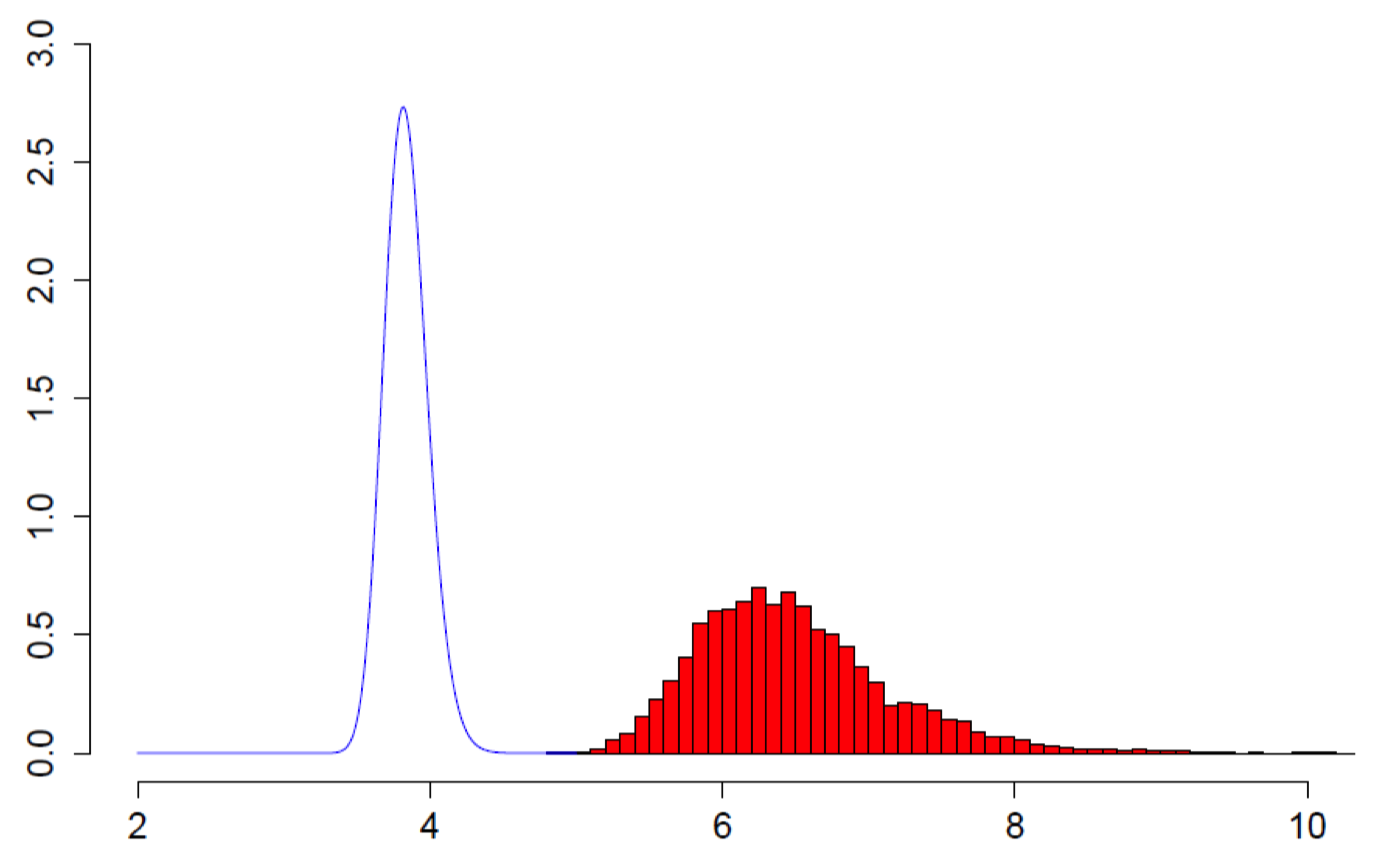
\includegraphics[width = 0.6 \textwidth]{figures/note18_resamplingfail.png}
    \caption{Failure of Resampling Test $(n=p=100)$}\label{fig:resampling_failure}
\end{figure}

Next, we develop another test to cope with these problems.

\section{Johnstone and Onatski (2020)}
Consider the basic equation of classical multivariate statistics:
\begin{align}
    \det \left( \mathbf{H}-\mathbf{xE}\right) = 0
\end{align}
with $p\times p$ matrices
\begin{align*}
    n_1\mathbf{H} &= \sum^{n_1}_{k=1}\mathbf{x}_k\mathbf{x}_k' &\text{\textit{hypothesis} SS}\\
    n_1\mathbf{E} &= \sum^{n_1}_{k=1}\mathbf{z}_k\mathbf{z}_k' &\text{\textit{error} SS}
\end{align*}
The solution $\mathbf{x}$ is generalized eigenvalues $\left\{ \lambda_i \right\}^p_{i=1}$, which are the eigenvalue of \myhl[myblue]{F-ratio} $\mathbf{E}^{-1}\mathbf{H}$. \citet{johnstone2020testing} summarized 5 topics using $\mathbf{E}^{-1}\mathbf{H}$ relying on the five most common hypergeometric functions\footnote{Hypergeometric functions are:
\begin{itemize}
\item scalar inputs $$ _{\mathrm{p}}\mathcal{F}_{\mathrm{q}}(a,b;x) = \sum^{\infty}_{k=0} \frac{(a_1)_k\cdots (a_p)_k}{(b_1)_k\cdots (b_p)_k}\frac{x^k}{k!} $$ where $(a_j)_k$ are generalized Pochhammer symbols
\item single matrix inputs, where $\mathbf{S}$ is symmetric and usually diagonal $$ _{\mathrm{p}}\mathcal{F}_{\mathrm{q}}(a,b;\mathbf{S}) = \sum^{\infty}_{k=0} \sum_{\kappa} \frac{(a_1)_{\kappa}\cdots (a_p)_{\kappa}}{(b_1)_{\kappa}\cdots (b_p)_{\kappa}}\frac{C_{\kappa}(\mathbf{S})}{k!}  $$ where $C_k$ are the zonal polynomials. Easily, $ _{\mathrm{0}}\mathcal{F}_{\mathrm{0}}(\mathbf{S}) = e^{\mathrm{tr}(\mathbf{S})}$, $ _{\mathrm{1}}\mathcal{F}_{\mathrm{0}}(a,\mathbf{S}) = \left\vert \mathbf{I-S} \right\vert^{-a}$
\item two matrix inputs, where $\mathbf{S,T}$ are both symmetric $$ _{\mathrm{p}}\mathcal{F}_{\mathrm{q}}(a,b;\mathbf{S,T})  = \int_{O(p)} _{\mathrm{p}}\mathcal{F}_{\mathrm{q}} (a,b;\mathbf{SUTU'})\mathrm(d)\mathbf{U} $$
\end{itemize} } $_{\mathrm{p}}\mathcal{F}_{\mathrm{q}}$

\begin{table}[ht]
    \footnotesize
    \begin{center}
      \begin{tabular}{lccccc}
        
        \multicolumn{3}{c}{Statistical method} & $n_1\mathbf{H}$ & $n_2\mathbf{E}$ & Univariate Analog \\
        \hline
        $_{\mathrm{0}}\mathcal{F}_{\mathrm{0}}$ & PCA & Principal components analysis & $W_p(n_1,\boldsymbol{\Sigma+\Phi})$ & $n_2\boldsymbol{\Sigma}$ & $\chi^2$\\
        $_{\mathrm{1}}\mathcal{F}_{\mathrm{0}}$ & SigD & Signal detection & $W_p(n_1,\boldsymbol{\Sigma+\Phi})$ & $W_p(n_2,\boldsymbol{\Sigma})$ & non-central $\chi^2$ \\
        $_{\mathrm{0}}\mathcal{F}_{\mathrm{1}}$ & REG$_0$ & Multivariate regression, with known error & $W_p(n_1,\boldsymbol{\Sigma},n_1\boldsymbol{\Phi})$ & $n_2\boldsymbol{\Sigma}$ & $F$ \\
        $_{\mathrm{1}}\mathcal{F}_{\mathrm{1}}$ & REG & Multivariate regression, with unknown error & $W_p(n_1,\boldsymbol{\Sigma},n_1\boldsymbol{\Phi})$ & $W_p(n_2,\boldsymbol{\Sigma})$ & non-central $F$ \\
        $_{\mathrm{2}}\mathcal{F}_{\mathrm{1}}$ & CCA & Canonical correlation analysis & $W_p(n_1,\boldsymbol{\Sigma},\boldsymbol{\Phi}(\mathbf{Y}))$ & $W_p(n_2,\boldsymbol{\Sigma})$ & $\frac{r^2}{1-r^2}$\\ \hline
        \multicolumn{5}{l}{For $_{\mathrm{0}}\mathcal{F}_{\mathrm{0}}$ and $_{\mathrm{0}}\mathcal{F}_{\mathrm{1}}$, $\mathbf{E}$ is deterministic, $\boldsymbol{\Sigma}$ is known, $n_2$ disppears, otherwise $\mathbf{E}$ is independent of $\mathbf{H}$.}
      \end{tabular}
    \end{center}
  \end{table}

\newpage
\bibliographystyle{plainnat}
\bibliography{ref.bib}

\end{document}